%Parameter Tuning
\subsection{Parameter Tuning}

This section describes the parameter tuning procedure for the Tabu Search algorithm. The goal of parameter tuning is to identify the best combination of algorithm parameters that minimizes the objective function value across diverse problem instances.

\subsubsection{Experimental Design}

The parameter tuning experiments were conducted on six representative Solomon benchmark instances: C101, C201 (clustered), R101, R201 (random), and RC101, RC201 (mixed). For each configuration, three independent runs were performed with different random seeds to ensure statistical robustness.

The following parameters were varied:
\begin{itemize}
    \item \textbf{Neighborhood operator}: swap, insert, invert.
    \item \textbf{Tabu List Size}: 10, 20, 30, 40, 50.
    \item \textbf{Number of Iterations}: 50, 100, 150, 200, 250, 300 -- representing the number of consecutive iterations without improvement after which the current solution is discarded and replaced with a new random solution.
\end{itemize}

This resulted in $3 \times 5 \times 6 = 90$ unique parameter configurations, each tested on all six instances with three repetitions, yielding a total of 1620 experimental runs.

\subsubsection{Results by Neighborhood operator}

Figure~\ref{fig:mutation_comparison} presents the comparison of mean objective values achieved by different neighborhood operators. The \texttt{swap} operator consistently outperforms both \texttt{insert} and \texttt{invert} operators across all tested configurations.

\begin{figure}[ht]
    \centering
    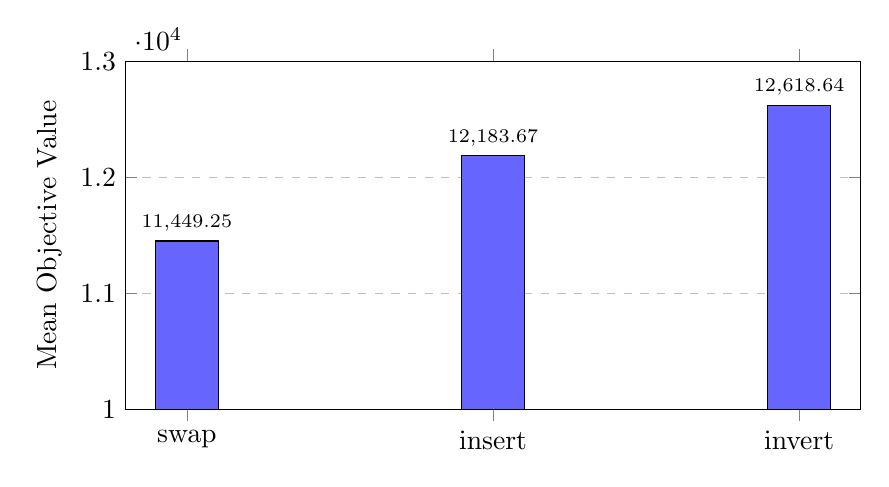
\begin{tikzpicture}
        \begin{axis}[
            ybar,
            bar width=0.8cm,
            width=0.9\columnwidth,
            height=6cm,
            ylabel={Mean Objective Value},
            symbolic x coords={swap, insert, invert},
            xtick=data,
            ymin=10000,
            ymax=13000,
            nodes near coords,
            nodes near coords align={vertical},
            every node near coord/.append style={font=\scriptsize, rotate=0},
            ymajorgrids=true,
            grid style=dashed,
        ]
        \addplot[fill=blue!60] coordinates {
            (swap, 11449.25)
            (insert, 12183.67)
            (invert, 12618.64)
        };
        \end{axis}
    \end{tikzpicture}
    \caption{Comparison of mean objective values by neighborhood operator. Lower values indicate better performance. The \texttt{swap} method achieves the lowest average objective value.}
    \label{fig:mutation_comparison}
\end{figure}

Table~\ref{tab:mutation_summary} provides statistics for each neighborhood operator. The \texttt{swap} operator not only achieves the lowest mean objective (11449.25) but also demonstrates the smallest variation, indicating more consistent performance.

\begin{table}[ht]
    \renewcommand{\arraystretch}{1.3}
    \caption{Summary statistics of objective values by neighborhood operator.}
    \label{tab:mutation_summary}
    \centering
    \begin{tabular}{l|c|c|c|c}
        \hline\hline
        Nbh & Mean & Min & Max & Improvement \\
        \hline\hline
        swap   & 11449.25 & 4981.76 & 25969.94 & 16.98\% \\ \hline
        insert & 12183.67 & 5415.28 & 27506.67 & 11.66\% \\ \hline
        invert & 12618.64 & 5077.71 & 29236.06 &  8.50\% \\
        \hline\hline
    \end{tabular}
\end{table}

\subsubsection{Impact of Tabu List Size}

Figure~\ref{fig:tabu_size_impact} shows the relationship between tabu list size and the mean objective value. The results indicate that larger tabu list sizes (40--50) tend to produce slightly better results, although the differences remain relatively small (less than 0.5\%).

\begin{figure}[ht]
    \centering
    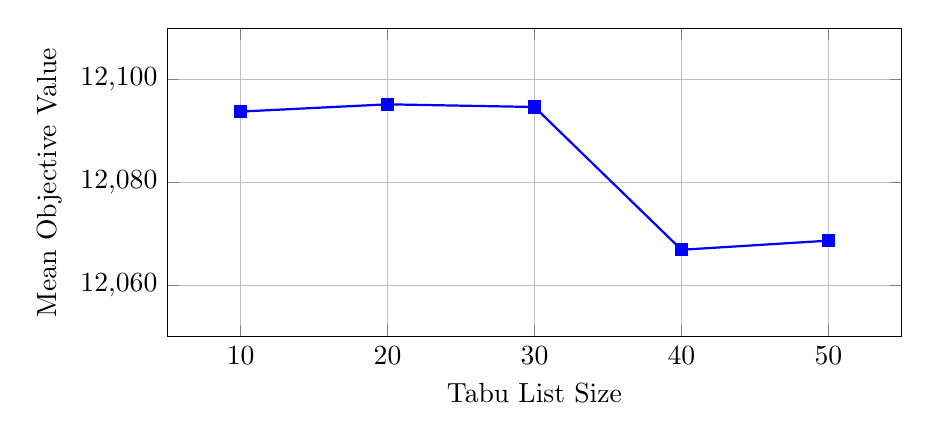
\begin{tikzpicture}
        \begin{axis}[
            width=0.9\columnwidth,
            height=5.5cm,
            xlabel={Tabu List Size},
            ylabel={Mean Objective Value},
            xmin=5,
            xmax=55,
            ymin=12050,
            ymax=12110,
            xtick={10,20,30,40,50},
            grid=both,
            grid style={line width=.1pt, draw=gray!30},
            major grid style={line width=.2pt,draw=gray!50},
            mark size=2pt,
            legend pos=north east,
            scaled y ticks = false,
        ]
        \addplot[color=blue, mark=square*, thick] coordinates {
            (10, 12093.79)
            (20, 12095.20)
            (30, 12094.68)
            (40, 12066.91)
            (50, 12068.69)
        };
        \end{axis}
    \end{tikzpicture}
    \caption{Impact of tabu list size on mean objective value. Larger tabu sizes (40--50) show marginally better performance.}
    \label{fig:tabu_size_impact}
\end{figure}

\subsubsection{Impact of Number of Iterations}

Figure~\ref{fig:iterations_impact} illustrates the effect of the \textit{no-improvement iteration limit}, i.e., the number of consecutive iterations without improvement after which a~new random solution is generated. Increasing this limit from 50 to 100--200 improves solution quality by allowing the algorithm to explore the current region of the search space more thoroughly. Beyond 200 iterations, improvements diminish, as excessively long stagnation periods delay potentially beneficial diversification.

\begin{figure}[ht]
    \centering
    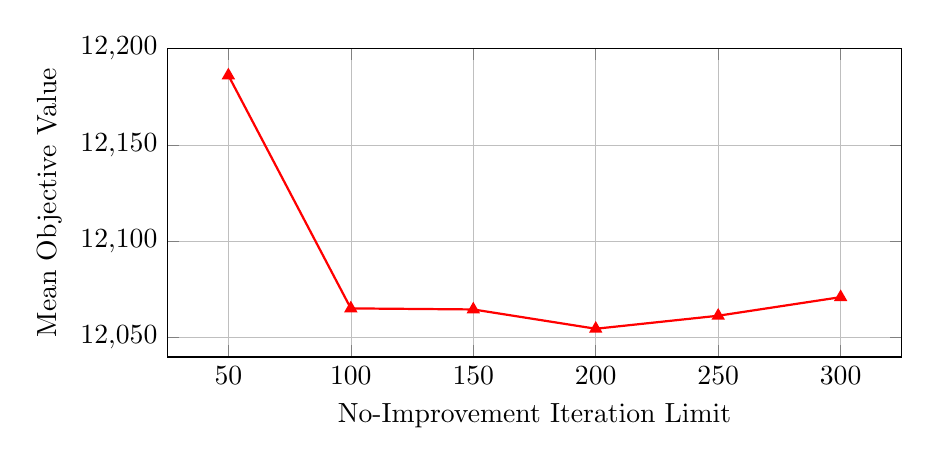
\begin{tikzpicture}
        \begin{axis}[
            width=0.9\columnwidth,
            height=5.5cm,
            xlabel={No-Improvement Iteration Limit},
            ylabel={Mean Objective Value},
            xmin=25,
            xmax=325,
            ymin=12040,
            ymax=12200,
            xtick={50,100,150,200,250,300},
            grid=both,
            grid style={line width=.1pt, draw=gray!30},
            major grid style={line width=.2pt,draw=gray!50},
            mark size=2pt,
            scaled y ticks = false,
        ]
        \addplot[color=red, mark=triangle*, thick] coordinates {
            (50, 12186.06)
            (100, 12065.22)
            (150, 12064.68)
            (200, 12054.67)
            (250, 12061.42)
            (300, 12071.06)
        };
        \end{axis}
    \end{tikzpicture}
    \caption{Impact of iteration limit on mean objective value. Performance improves significantly from 50 to 100--200 iterations, with diminishing returns beyond 200.}
    \label{fig:iterations_impact}
\end{figure}

\subsubsection{Best Configuration}

Table~\ref{tab:best_configs} summarizes the best parameter configurations identified for each neighborhood operator. The overall best configuration uses the \texttt{swap} operator with tabu size of 50 and a no-improvement limit of 100 iterations, achieving a mean objective value of 11263.33.

\begin{table}[ht]
    \renewcommand{\arraystretch}{1.3}
    \caption{Best parameter configurations for each neighborhood operator.}
    \label{tab:best_configs}
    \centering
    \begin{tabular}{l|c|c|c}
        \hline\hline
        Nbh & Tabu Size & No-Improvement Limit & Mean Objective \\
        \hline\hline
        swap   & 50 & 100 & \textbf{11263.33} \\ \hline
        insert & 40 & 150 & 12138.55 \\ \hline
        invert & 10 & 250 & 12407.64 \\
        \hline\hline
    \end{tabular}
\end{table}

% \subsubsection{Conclusions from Parameter Tuning}

The parameter tuning experiments lead to the following conclusions:

\begin{enumerate}
    \item \textbf{neighborhood operator}: The \texttt{swap} move significantly outperforms \texttt{insert} and \texttt{invert}, providing 6--10\% lower objective values on average.

    \item \textbf{Tabu list size}: Larger tabu sizes (40--50) yield slightly better performance by reducing premature cycling, although differences remain small.

    \item \textbf{Iteration limit}: Allowing 100--200 consecutive non-improving iterations leads to the best results, as it balances intensification and diversification. Lower limits terminate the search too early, while higher limits introduce unnecessary stagnation.

    \item \textbf{Recommended configuration}: For subsequent experiments, the recommended configuration is the \texttt{swap} operator, tabu size of 30, and a no-improvement limit of 100 iterations. Although the absolute best performance was obtained with tabu size 50, the difference is marginal, and the smaller tabu size provides better computational efficiency.
\end{enumerate}

These findings guided the parameter selection for the main experimental evaluation described in the following subsections.
